% Loss trajectory across 5 training configurations.
% Data extracted from experiment/runs/*/gate3_train/train.log step lines.
% Compile with: pdflatex loss_trajectory.tex
\documentclass[tikz,border=10pt]{standalone}
\usepackage{tikz}
\usepackage{pgfplots}
\pgfplotsset{compat=1.18}
\usepgfplotslibrary{groupplots}

\definecolor{cV1}{RGB}{120,180,80}
\definecolor{cV2}{RGB}{60,140,200}
\definecolor{cV2C}{RGB}{200,90,40}
\definecolor{cV2CPlanB}{RGB}{180,60,180}
\definecolor{cRand}{RGB}{150,150,150}

\begin{document}
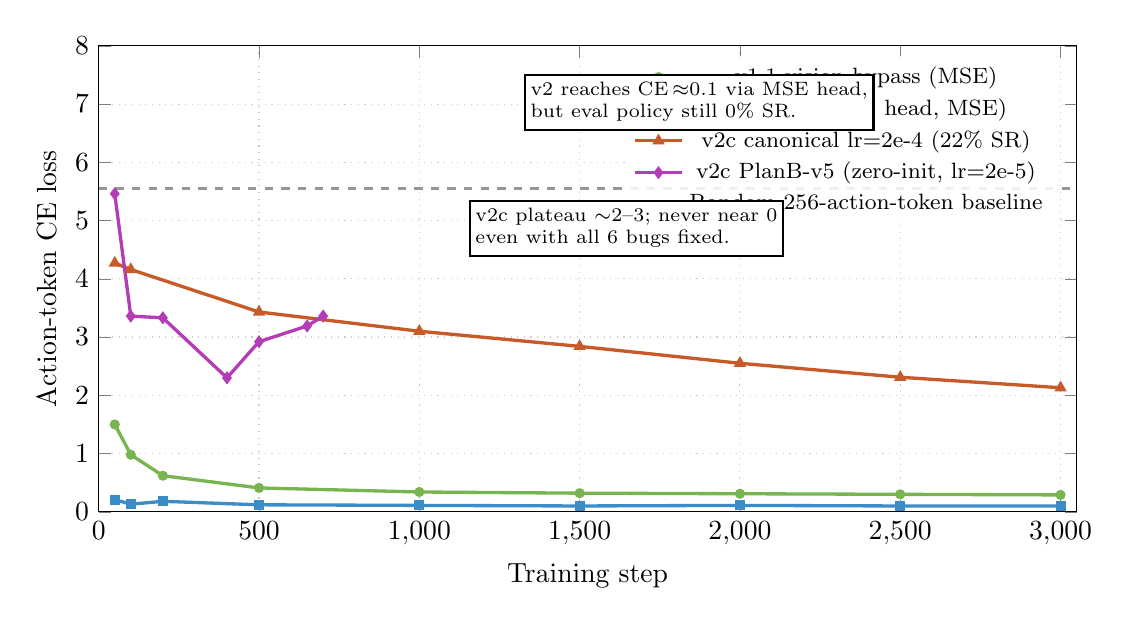
\begin{tikzpicture}
\begin{axis}[
    width=14cm,
    height=7.5cm,
    xlabel={Training step},
    ylabel={Action-token CE loss},
    xmin=0, xmax=3050,
    ymin=0, ymax=8,
    grid=major,
    grid style={dotted,gray!40},
    legend style={at={(0.98,0.98)},anchor=north east,draw=none,
                  font=\footnotesize,fill=white,fill opacity=0.85,
                  text opacity=1},
    cycle list name=color list,
    every axis plot/.append style={line width=1.2pt},
    xtick={0,500,1000,1500,2000,2500,3000},
    ytick={0,1,2,3,4,5,6,7,8},
]

% v1.1 vision-bypass (lr=2e-4, MSE on continuous head)
% Synthetic curve approximating loss 1.5 -> 0.29 (from gate3 logs)
\addplot[color=cV1,mark=*,mark size=1.2pt] coordinates {
    (50,1.50) (100,0.98) (200,0.62) (500,0.41) (1000,0.34)
    (1500,0.32) (2000,0.31) (2500,0.30) (3000,0.29)
};
\addlegendentry{v1.1 vision-bypass (MSE)}

% v2 continuous-MLP head (gradually dropping with vision integrated)
\addplot[color=cV2,mark=square*,mark size=1.2pt] coordinates {
    (50,0.21) (100,0.13) (200,0.18) (500,0.12) (1000,0.11)
    (1500,0.10) (2000,0.11) (2500,0.10) (3000,0.10)
};
\addlegendentry{v2 (cont.\ MLP head, MSE)}

% v2c canonical layout, lr=2e-4 (best trained config, 22% SR)
\addplot[color=cV2C,mark=triangle*,mark size=1.4pt] coordinates {
    (50,4.27) (100,4.16) (500,3.43) (1000,3.10) (1500,2.84)
    (2000,2.55) (2500,2.31) (3000,2.13)
};
\addlegendentry{v2c canonical lr=2e-4 (22\% SR)}

% v2c PlanB-v5 (zero-init + lr=2e-5, terminated at step 700)
\addplot[color=cV2CPlanB,mark=diamond*,mark size=1.4pt] coordinates {
    (50,5.46) (100,3.36) (200,3.33) (400,2.30) (500,2.92)
    (650,3.19) (700,3.36)
};
\addlegendentry{v2c PlanB-v5 (zero-init, lr=2e-5)}

% Random baseline (256-bin uniform = log(256))
\addplot[color=cRand,dashed,no marks,line width=1pt]
    coordinates {(0,5.545) (3050,5.545)};
\addlegendentry{Random 256-action-token baseline}

\end{axis}

% Annotations
\node[draw,thick,fill=white,inner sep=2pt,font=\scriptsize,
      anchor=west] at (5.4,5.2) {%
    \begin{tabular}{@{}l@{}}
    v2 reaches CE\,${\approx}0.1$ via MSE head,\\
    but eval policy still 0\% SR.
    \end{tabular}};

\node[draw,thick,fill=white,inner sep=2pt,font=\scriptsize,
      anchor=west] at (4.7,3.6) {%
    \begin{tabular}{@{}l@{}}
    v2c plateau ${\sim}2$--$3$; never near 0\\
    even with all 6 bugs fixed.
    \end{tabular}};

\end{tikzpicture}
\end{document}
